% По умолчанию используется шрифт 14 размера. Если нужен 12-й шрифт, уберите опцию [14pt]
\documentclass[14pt
  , russian
  %, xcolor={svgnames}
  ]{matmex-diploma-custom}
\usepackage[table]{xcolor}
\usepackage{graphicx}
\usepackage{tabularx}
\newcolumntype{Y}{>{\centering\arraybackslash}X}
\usepackage{amsmath}
\usepackage{amsthm}
\usepackage{amsfonts}
\usepackage{amssymb}
\usepackage{mathtools}
\usepackage{thmtools}
\usepackage{thm-restate}
\usepackage{tikz}
\usepackage{wrapfig}
% \usepackage[kpsewhich,newfloat]{minted}
% \usemintedstyle{vs}
\usepackage[inline]{enumitem}
\usepackage{subcaption}
\usepackage{caption}
\usepackage[nocompress]{cite}
\usepackage{makecell}
% \setitemize{noitemsep,topsep=0pt,parsep=0pt,partopsep=0pt}
% \setenumerate{noitemsep,topsep=0pt,parsep=0pt,partopsep=0pt}


\graphicspath{ {resources/} }

% 
% % \documentclass 
% %   [ a4paper        % (Predefined, but who knows...)
% %   , draft,         % Show bad things.
% %   , 12pt           % Font size.
% %   , pagesize,      % Writes the paper size at special areas in DVI or
% %                    % PDF file. Recommended for use.
% %   , parskip=half   % Paragraphs: noindent + gap.
% %   , numbers=enddot % Pointed numbers.
% %   , BCOR=5mm       % Binding size correction.
% %   , submission
% %   , copyright
% %   , creativecommons 
% %   ]{eptcs}
% % \providecommand{\event}{ML 2018}  % Name of the event you are submitting to
% % \usepackage{breakurl}             % Not needed if you use pdflatex only.
% 
% \usepackage{underscore}           % Only needed if you use pdflatex.
% 
% \usepackage{booktabs}
% \usepackage{amssymb}
% \usepackage{amsmath}
% \usepackage{mathrsfs}
% \usepackage{mathtools}
% \usepackage{multirow}
% \usepackage{indentfirst}
% \usepackage{verbatim}
% \usepackage{amsmath, amssymb}
% \usepackage{graphicx}
% \usepackage{xcolor}
% \usepackage{url}
% \usepackage{stmaryrd}
% \usepackage{xspace}
% \usepackage{comment}
% \usepackage{wrapfig}
% \usepackage[caption=false]{subfig}
% \usepackage{placeins}
% \usepackage{tabularx}
% \usepackage{ragged2e}
% \usepackage{soul}
\usepackage{csquotes}
% \usepackage{inconsolata}
% 
% \usepackage{polyglossia}   % Babel replacement for XeTeX
%   \setdefaultlanguage[spelling=modern]{russian}
%   \setotherlanguage{english}
% \usepackage{fontspec}    % Provides an automatic and unified interface 
%                          % for loading fonts.
% \usepackage{xunicode}    % Generate Unicode chars from accented glyphs.
% \usepackage{xltxtra}     % "Extras" for LaTeX users of XeTeX.
% \usepackage{xecyr}       % Help with Russian.
% 
% %% Fonts
% \defaultfontfeatures{Mapping=tex-text}
% \setmainfont{CMU Serif}
% \setsansfont{CMU Sans Serif}
% \setmonofont{CMU Typewriter Text}

\usepackage[final]{listings}

\lstdefinelanguage{ocaml}{
keywords={@type, function, fun, let, in, match, with, when, class, type,
nonrec, object, method, of, rec, repeat, until, while, not, do, done, as, val, inherit, and,
new, module, sig, deriving, datatype, struct, if, then, else, open, private, virtual, include, success, failure,
lazy, assert, true, false, end},
sensitive=true,
commentstyle=\small\itshape\ttfamily,
keywordstyle=\ttfamily\bfseries, %\underbar,
identifierstyle=\ttfamily,
basewidth={0.5em,0.5em},
columns=fixed,
fontadjust=true,
literate={->}{{$\to$}}3 {===}{{$\equiv$}}1 {=/=}{{$\not\equiv$}}1 {|>}{{$\triangleright$}}3 {\\/}{{$\vee$}}2 {/\\}{{$\wedge$}}2 {>=}{{$\ge$}}1 {<=}{{$\le$}} 1,
morecomment=[s]{(*}{*)}
}

\lstset{
mathescape=true,
%basicstyle=\small,
identifierstyle=\ttfamily,
keywordstyle=\bfseries,
commentstyle=\scriptsize\rmfamily,
basewidth={0.5em,0.5em},
fontadjust=true,
language=ocaml
}
 
\newcommand{\cd}[1]{\texttt{#1}}
\newcommand{\inbr}[1]{\left<#1\right>}


\newcolumntype{L}[1]{>{\raggedright\let\newline\\\arraybackslash\hspace{0pt}}m{#1}}
\newcolumntype{C}[1]{>{\centering\let\newline\\\arraybackslash\hspace{0pt}}m{#1}}
\newcolumntype{R}[1]{>{\raggedleft\let\newline\\\arraybackslash\hspace{0pt}}m{#1}}



\usepackage{soul}
\usepackage[normalem]{ulem}
%\sout{Hello World}

% перевод заголовков в листингах
\renewcommand\lstlistingname{Листинг}
\renewcommand\lstlistlistingname{Листинги}

\usepackage{afterpage}
\usepackage{pdflscape}
\usepackage{listings}
\usepackage{tikz}
\usetikzlibrary{decorations.pathreplacing,calc,shapes,positioning,tikzmark}

\newcounter{tmkcount}

\tikzset{
  use tikzmark/.style={
    remember picture,
    overlay,
    execute at end picture={
      \stepcounter{tmkcount}
    },
  },
  tikzmark suffix={-\thetmkcount}
}

\usepackage{caption}
\usepackage{listings}
\usepackage{graphicx}
\usepackage{multirow}
\usepackage{fancyvrb}
\usepackage[misc,geometry]{ifsym} 
\usepackage{subcaption}
\usepackage{multirow}
\usepackage{array}
\newcolumntype{P}[1]{>{\centering\arraybackslash}p{#1}}
\usepackage{tikz}
\usepackage{bbding}
\usepackage{pifont}
\usepackage{wasysym}
\usepackage{amssymb}
\usepackage{listings}
\usepackage{pythonhighlight}
\usepackage{tabularx}
\usepackage{array}
\newtheorem{definition}{Определение}

\DeclareCaptionFont{white}{ \color{white} }
\DeclareCaptionFormat{listing}{
    \parbox{\textwidth}{\hspace{15pt}#1#2#3}
}
\captionsetup[lstlisting]{ format=listing
  %, labelfont=white, textfont=white
  , singlelinecheck=false, margin=0pt, font={bf}
}

\setlength\extrarowheight{7pt}

\begin{document}
% Титульный лист (ГОСТ Р 7.0.11-2001, 5.1)
\thispagestyle{empty}
\begin{center}
\thesisOrganization
\end{center}
%
\vspace{0pt plus4fill} %число перед fill = кратность относительно некоторого расстояния fill, кусками которого заполнены пустые места
\IfFileExists{images/SPbGU_Logo.png}{
  \begin{minipage}[b]{0.5\linewidth}
    \begin{flushleft}
      
\includegraphics[height=3.5cm]{SPbGU_Logo}
    \end{flushleft}
  \end{minipage}%
  \begin{minipage}[b]{0.5\linewidth}
    \begin{flushright}
      На правах рукописи\\
%      \textsl {УДК \thesisUdk}
    \end{flushright}
  \end{minipage}
}{
\begin{flushright}
На правах рукописи

%\textsl {УДК \thesisUdk}
\end{flushright}
}
%
\vspace{0pt plus6fill} %число перед fill = кратность относительно некоторого расстояния fill, кусками которого заполнены пустые места
\begin{center}
{\large \thesisAuthor}
\end{center}
%
\vspace{0pt plus1fill} %число перед fill = кратность относительно некоторого расстояния fill, кусками которого заполнены пустые места
\begin{center}
\textbf {\large %\MakeUppercase
\thesisTitle}

\vspace{0pt plus2fill} %число перед fill = кратность относительно некоторого расстояния fill, кусками которого заполнены пустые места
{%\small
Специальность \thesisSpecialtyNumber\ "---

<<\thesisSpecialtyTitle>>
}

\ifdefined\thesisSpecialtyTwoNumber
{%\small
Специальность \thesisSpecialtyTwoNumber\ "---

<<\thesisSpecialtyTwoTitle>>
}
\fi

\vspace{0pt plus2fill} %число перед fill = кратность относительно некоторого расстояния fill, кусками которого заполнены пустые места
Диссертация на соискание учёной степени

\thesisDegree
\end{center}
%
\vspace{0pt plus4fill} %число перед fill = кратность относительно некоторого расстояния fill, кусками которого заполнены пустые места
\begin{flushright}
\ifdefined\supervisorTwoFio
Научные руководители:

\supervisorRegalia

\ifdefined\supervisorDead
\framebox{\supervisorFio}
\else
\supervisorFio
\fi

\supervisorTwoRegalia

\ifdefined\supervisorTwoDead
\framebox{\supervisorTwoFio}
\else
\supervisorFio
\fi
\else
Научный руководитель:

\supervisorRegalia

\ifdefined\supervisorDead
\framebox{\supervisorFio}
\else
\supervisorFio
\fi
\fi

\end{flushright}
%
\vspace{0pt plus4fill} %число перед fill = кратность относительно некоторого расстояния fill, кусками которого заполнены пустые места
{\centering\thesisCity\ "--- \thesisYear\par}

\maketitle
\setcounter{tocdepth}{2}
\tableofcontents

% \begin{abstract}
%   В курсаче не нужен
% \end{abstract}

\section{Введение}
Среди множества направлений научных исследований, которое охватывает вычислительная биология, особое место занимают различные прикладные задачи, связанные с анализом последовательностей, входящих в состав важнейших для всех живых организмов макромолекул --- ДНК, РНК и белков. Процесс разработки и оптимизации алгоритмов для решения целого ряда задач, например, классификации организмов, расшифровки геномов, предсказания функций белков и других, не прекращается уже много лет, и за это время были выработаны некоторые общие принципы работы с биологическими данными.

Во-первых, линейная (первичная) и пространственная (вторичная) структуры этих макромолекул содержат важную информацию о клеточных функциях и эволюционном происхождении организмов и могут быть формально описаны с помощью различных математических моделей. В частности, первичная структура молекулы РНК представляет собой цепочку особых веществ --- нуклеотидов, --- и в том случае, когда два фрагмента этой цепи соединяются друг с другом, перегибаясь и образуя на конце неспаренный участок в форме петли, формируется элемент, называемый в биологии шпилькой. Совокупность вложенных шпилек разных размеров составляет сложную и стабильную вторичную структуру. Известно, что вторичная структура играет важную роль в регуляции клеточных процессов~\cite{vandivier2016conservation}, поэтому во многих геномных исследованиях требуется учитывать или предсказывать ее конфигурацию. Существуют различные методы формального описания вторичной структуры, например, скрытые марковские модели~\cite{yoon2004hmm}, ковариационные модели~\cite{sippl1999biological} и формальные грамматики~\cite{dowell2004evaluation,knudsen1999rna,rivas2000language}.

Во-вторых, при работе с биологическими данными важно учитывать их потенциальную зашумленность, т.е. присутствие различных неточностей, мутаций и случайных всплесков, и, кроме того, законы образования пространственных молекулярных структур сами по себе имеют стохастическую природу. Поэтому в данной области у точных алгоритмов зачастую выигрывают те, что предполагают некоторого рода вероятностную оценку. Популярным способом обработки зашумленных данных являются методы машинного обучения, в частности, нейронные сети, которые в настоящее время успешно используются в том числе и в биоинформатике~\cite{higashi2009bacteria,sherman2017humidor}.

В рамках предыдущей дипломной работы был разработан подход для решения задач обработки последовательностей, обладающих некоторой синтаксической структурой. Данный подход основан на комбинировании методов синтаксического анализа и машинного обучения и может быть применен в совершенно разных предметных областях. Предлагается использовать формальную грамматику для кодирования характерных элементов синтаксической структуры, алгоритм синтаксического анализа --- для их поиска во входных данных, а обработку информации о наличии и расположении этих элементов в цепочке и вероятностную оценку провести с помощью нейронной сети, которая некоторым образом обрабатывает сгенерированные парсером данные. Анализ геномных последовательностей является одной из потенциальных областей применения этого подхода и, если говорить непосредственно об исследовании РНК, то входными данными являются нуклеотидные цепочки, под синтаксической структурой следует понимать вторичную структуру РНК, а под искомыми характерными элементами --- составляющие ее шпильки. 

Направлением исследования, представленного в данной работе, является предсказание вторичной структуры РНК с использованием описанного выше подхода. Правила контекстно-свободной грамматики описывают определенный по некоторым эмпирическим критериям общий вид шпилек вторичной структуры, а синтаксический анализатор выполняет задачу поиска подстроки в строке, что с теоретической точки зрения означает получение всех выводимых по правилам грамматики подстрок, а с практической --- всех потенциально возможных в данной строке шпилек. Однако в контексте реальной вторичной структуры РНК живого организма эта информация является избыточной, так как из всех возможных комбинаций шпилек будет присутствовать только какая-то одна, а иногда и недостаточной, потому что грамматика не может не содержать определенные ограничения, например, на максимальный размер петли внутри шпильки. Поэтому для генерации чистой вторичной структуры из результата работы парсера в рамках рассматриваемого подхода предлагается использовать нейронную сеть, задача которой в данном случае --- отфильтровать лишние шпильки и достроить невыразимые в грамматике элементы.

\section{Постановка задачи}
\label{sec:task}
Целью данной работы является исследование возможности применения подхода, основанного на комбинировании методов синтаксического анализа и машинного обучения, к задаче предсказания вторичной структуры молекулы РНК. Для реализации данной цели были поставлены следующие задачи.
\begin{itemize}
    \item Разработка архитектуры решения, конкретизирующей форматы анализируемых данных, а также используемые формальные грамматики и нейронные сети.
    \item Проведение экспериментальных исследований предложенной архитектуры, сравнение полученных результатов с существующими решениями.
\end{itemize}

\section{Обзор}
\label{sec:relatedworks}
\subsection{Описание предметной области}
Входящие в состав клеток всех живых существ макромолекулы --- нуклеиновые кислоты и белки --- имеют очень разнообразные биологические функции и играют важные роли во множестве процессов, определяющих жизнедеятельность и эволюционное развитие организмов. Со структурной точки зрения их объединяет то, что они являются полимерами, т.е. состоят из некоторых элементарных единиц --- мономеров, --- соединенных в крупные молекулы по определенным законам.  Как ДНК и РНК, так и белки имеют несколько уровней организации, т.е. характеризуются линейной (первичной) структурой, которая представляет собой последовательность из мономеров, и пространственной (вторичной), основанной на молекулярных взаимодействиях между ними. 

В частности, молекула РНК состоит из цепи особых веществ --- нуклеотидов четырех типов, которые называются аденин, гуанин, цитозин и урацил (A, G, C, U) и могут образовывать между собой попарные водородные связи. Законы формирования нуклеотидных пар обусловлены поддержанием термодинамического равновесия вторичной структуры, и самыми стабильными и распространенными в природе являются канонические, Уотсон-Криковские, пары $A-U$, $C-G$, однако с разной степенью вероятности могут встречаться и любые другие комбинации. Способность нуклеотидов формировать связи приводит к склеиванию определенных участков цепи РНК между собой и образованию вторичной структуры, базовым элементом которой является так называемая шпилька, которая образуется в том случае, когда две последовательности одной и той же цепи соединяются друг с другом, перегибаясь одна к другой и образуя на конце неспаренный участок --- петлю. Пример элементарной шпильки высоты четыре, образованной только каноническими парами, показан на рис.~\ref{rna_a}, и вторичная структура РНК в целом может быть представлена как рекурсивная композиция шпилек варьирующегося размера~\cite{quadrini2019loop}. В различных работах по биоинформатике можно встретить разделение элементов вторичной структуры по внешнему виду на несколько типов (hairpin, internal loop, bulge, helix, multi-loop и др.), однако формально все эти элементы могут быть определены через вложенные шпильки (рис.~\ref{rna_b}). Особый интерес представляют псевдоузлы (pseudoknots), состоящие из двух шпилек, где половина стебля одной из них располагается между двумя половинами стебля другой, и имеющее большое функциональное значение для живых организмов. 

\begin{figure}[h]
\centering
\begin{subfigure}{.5\textwidth}
  \centering
  \fbox{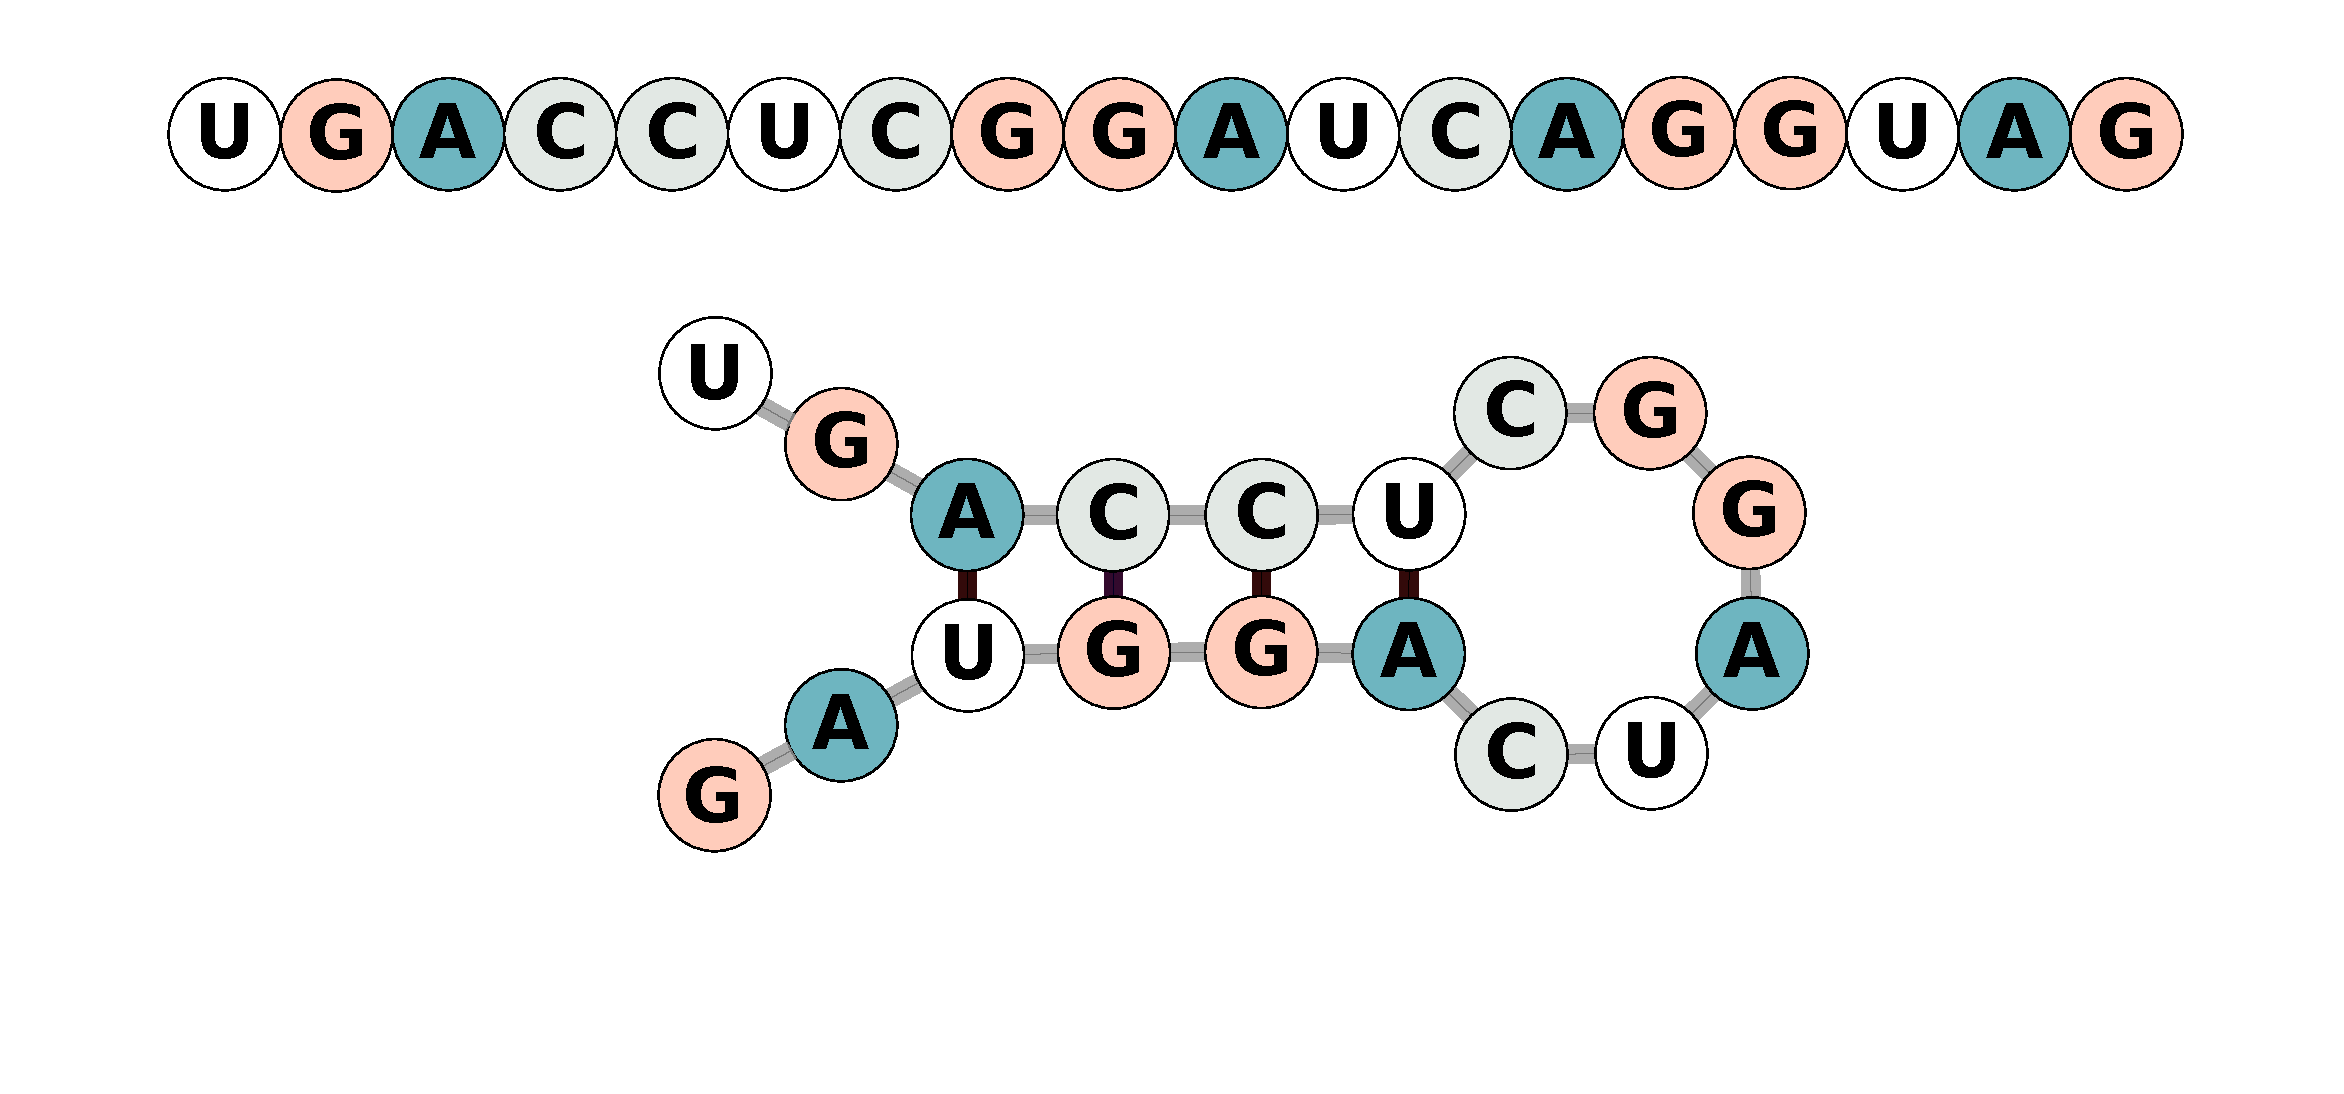
\includegraphics[width=7.7cm]{pics/stem.pdf}}
  \caption{Простая шпилька}
  \label{rna_a}
\end{subfigure}%
\begin{subfigure}{.5\textwidth}
  \centering
  \fbox{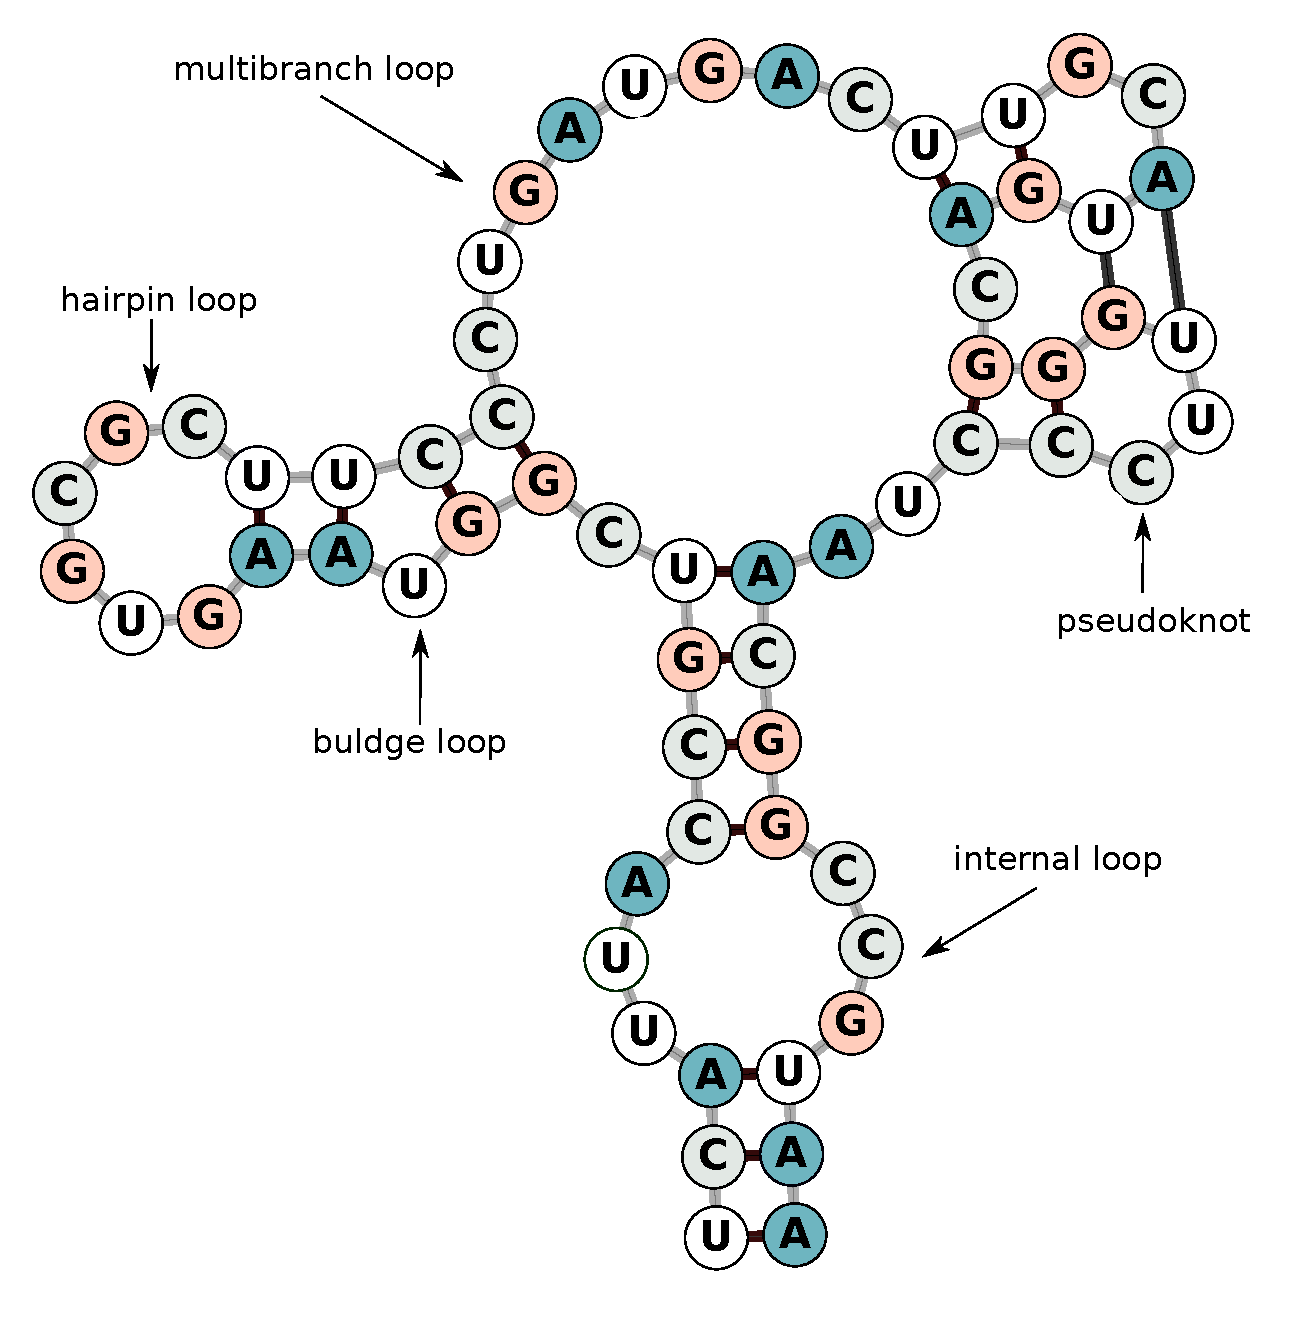
\includegraphics[width=7.7cm]{pics/rna.pdf}}
  \caption{Многообразие элементов}
  \label{rna_b}
\end{subfigure}
\caption{Вторичная структура РНК}
\label{rna}
\end{figure}

Различные исследования свойств и особенностей вторичной структуры РНК показали, что она активно участвует в таких процессах регуляции генома, как транскрипция и трансляция~\cite{wada1986local}, а также играет важную роль для филогенетического и таксономического анализа последовательностей~\cite{vrehakova2014variation,miladi2017rnascclust}, поэтому точное предсказание вторичной структуры РНК по ее нуклеотидной цепи относится к ключевым задачам современной геномики, которая усложняется тем, что вторичная структура обладает широкой вариативностью и в большинстве случаев не описывается исключительно через композицию простых шпилек, образованных Уотсон-Криковскими парами, а содержит более нетривиальные элементы.

\subsection{Подходы к предсказанию вторичной структуры РНК}
Существует большое количество  методов для предсказания вторичной структуры РНК, основанных на совершенно разных концепциях и технологиях. Самыми точными являются результаты, полученные в лабораторных условиях, например с помощью рентгеноструктурного анализа~\cite{westhof2015twenty} или ядерного магнитного резонанса~\cite{furtig2003nmr}, тем не менее, высокая цена и сложность постановки таких экспериментов приводят к активному развитию альтернативных методов --- вычислительных.

Вычислительные методы предсказания вторичных структур можно поделить на две основные группы. К первой относятся техники сравнительного анализа гомологичных последовательностей, основанные на идее о том, что биологически важные вторичные структуры не сильно меняются в процессе эволюции, поэтому сохранение двух довольно удаленных друг от друга нуклеотидов указывает на наличие водородной связи между ними во вторичной структуре~\cite{gutell2002accuracy,chen1999rna}. Такого рода результаты представляются достаточно надежными и часто используются в качестве эталонных в различных экспериментах, однако данный подход требует значительного объема ручной работы по выравниванию последовательностей и наличия достаточного количества родственных РНК для каждого вида, что далеко не всегда реализуемо на практике. Вторая и наиболее интересная в рамках данной работы группа объединяет все методы, предсказывающие вторичную структуру для единичной последовательности РНК путем построения некоторой описывающей ее физической или математической модели и решения проблемы ее оптимизации. 
Одним из самых популярных здесь подходов является принцип минимизации свободной энергии, основанный на требовании термодинамической стабильности вторичной структуры. Для решения задачи минимизации энергии могут применяться разные техники, в частности, динамическое программирование~\cite{bellaousov2013rnastructure,rivas1999dynamic}, эвристические алгоритмы~\cite{ren2005hotknots,ruan2004ilm} или иные оптимизационные схемы~\cite{reeder2007pknotsrg, jabbari2018knotty}. Кроме того, существует ряд методов, не основанных на физически измеряемых параметрах, в частности, часто максимизируется на всем пространстве вторичных структур некоторая функция оценки точности предсказания~\cite{hamada2009prediction,sato2009centroidfold} или используются стохастические контекстно-свободные грамматики для вероятностного моделирования вторичной структуры~\cite{knudsen1999rna,dowell2004evaluation}. 

Теоретическое понимание механизмов свертки последовательностей РНК и практическая реализация соответствующей модели являются достаточно нетривиальными задачами, что стало поводом к активному внедрению различных техник машинного обучения в процесс разработки алгоритмов предсказания вторичных структур как в качестве способа оценки оптимизируемых строгим алгоритмом параметров~\cite{akiyama2018max,do2006contrafold}, так и в качестве основного используемого метода~\cite{singh2019rna,apolloni2003rna}.

Несмотря на быстрое развитие идей и технологий в области вычислительной геномики, на данный момент проблема предсказания вторичной структуры молекулы РНК остается открытой, и основными сложностями при разработке алгоритмов являются предсказание псевдоузлов, неканонических пар оснований и обработка длинных последовательностей.

\subsection{Используемые технологии}
Предлагаемый в данной работе подход основан на комбинировании методов синтаксического анализа и машинного обучения, и в данном разделе будут введены основные используемые далее понятия из этих двух областей.

\subsubsection{Синтаксический анализ}
Алфавитом называется любое конечное непустое множество символов, и если $V$ --- алфавит, то через $V^\ast$ обозначается множество всех строк, составленных из символов $V$, а $L \subseteq V^\ast$  называется языком над алфавитом $V$. Для описания структуры конкретного языка, т.е. для выделения определенного подмножества из множества всех строк заданного алфавита, используется абстракция, именуемая грамматикой.

В задании правил грамматики участвуют терминальные символы, т.е. элементарные единицы некоторого языка, и нетерминальные --- синтаксические переменные, которые могут быть заменены группами терминальных символов. Формально, грамматикой называется четверка $G = (V_T, V_N, P, S)$, где $V_T$ ---  алфавит терминалов, $V_N$ --- алфавит нетерминалов, через $P$ обозначается конечное множество правил вида $\alpha \rightarrow \beta$, где $\alpha \in V^\ast V_N V^\ast$, $\beta \in V^\ast$, $V = V_N \cup V_T$, а $S$ --- стартовый нетерминал грамматики, т.е. тот нетерминал, из которого могут быть получены все предложения задаваемого ей языка. В теории формальных языков описаны различные классы грамматик, и в данной работе интерес для нас будут представлять контекстно-свободные грамматики, в которых для каждого правила $\alpha \rightarrow \beta$ выполняется условие $\alpha \in V_N$.

Строка $w$ называется выводимой из нетерминального символа $N$ грамматики $G$, если $w$ может быть получена из $N$ путем применения некоторой последовательности правил из множества правил $P$. Для автоматизации проверки выводимости строк используются различные алгоритмы синтаксического анализа, среди которых важное место занимают табличные алгоритмы, в процессе работы заполняющие для строки $w$ и нетерминала грамматики $N$ особую матрицу --- матрицу разбора $M_N$, в которой $M_N[i][j] = 1$ тогда и только тогда, когда подстрока $w[i..j]$ выводима из $N$. Самым известным табличным алгоритмом, работающим с контекстно-свободными грамматиками, является CYK~\cite{cocke1969programming,younger1967recognition,kasami1966efficient}, на ключевых принципах работы которого основываются и многие современные алгоритмы.

В рамках исследовательского проекта YaccConstructor~\cite{yacc} лаборатории языковых
инструментов JetBrains~\cite{jetbrains} проводятся исследования в области формальных языков. Среди прочего, в рамках данного проекта разрабатываются различные алгоритмы синтаксического анализа, и в данной работе использован алгоритм, основанный на матричных операциях~\cite{azimov2018context}, который демонстрирует высокую производительность на практике в связи с использованием параллельных вычислений.

\subsubsection{Машинное обучение}
К машинному обучению относятся методы создания компьютерных систем, способных находить закономерности в больших объемах данных через некоторым образом организованный процесс самостоятельного обучения. Один из таких методов --- нейронные сети --- повсеместно применяется в науке и технике, и концептуальной основой для построения обучаемой математической модели в данном случае являются принципы работы нейронов человеческого мозга.

При проектировании нейросети в первую очередь следует определить ее архитектуру, и одной из классических архитектур являются сверточные нейронные сети (convolutional neural networks), обрабатывающие, как правило, различного рода изображения. Такие сети работают на основе фильтров, которые отвечают за распознавание определенных характеристик изображения. Фильтр --- это коллекция ядер свертки, т.е. небольших матриц из чисел (весов), которые заранее неизвестны и устанавливаются в процессе обучения. Такие матрицы обрабатывают изображения по фрагментам с целью обнаружения искомых характеристик, осуществляя операцию свертки, которая является суммой произведений элементов фильтра и матрицы входных сигналов. Для решения сложных задач с многоуровневым выявлением признаков на практике требуются многослойные сверточные сети, которые часто оказывается затруднительно оптимизировать --- с увеличением глубины начинает падать точность вследствие особенностей алгоритмов обновления весов. Для решения этой проблемы была предложена особая архитектура --- остаточные нейронные сети (residual neural networks)~\cite{he2016deep}, --- основанная на добавлении дополнительных соединений быстрого доступа между блоками слоев, что упрощает процесс обучения на начальных этапах и позволяет улучшать точность результата с увеличением глубины. 

Помимо архитектуры, важным аспектом разработки нейронной сети является определение минимизируемой в процессе обучения функции ошибки (loss function), а также подбор оптимальных гиперпараметров, к которым относятся число слоев и нейронов в них, коэффициент скорости обучения (learning rate), число итераций обучения, функция активации, размер батча, способ разделения данных на обучающую и тестовую выборки и т.д. Качество работы нейросети оценивается по результатам вычисления различных метрик на тестовой выборке.

Существует множество платформ для создания и обучения нейронных сетей, и в данной работе были использованы написанные на языке Python библиотека Keras~\cite{chollet2015keras} и фреймворк Tensorflow~\cite{tensorflow2015-whitepaper}, так как данные технологии сочетают в себе удобство использования и высокую производительность.


\section{Архитектура решения}
\begin{frame}[fragile]
	\transwipe[direction=90]
	\frametitle{\faCogs\ Модернизация архитектуры}
	
	\begin{columns}
        \begin{column}{0.5\textwidth}
            \begin{figure}[hbt!]{\textwidth}
				\centering
				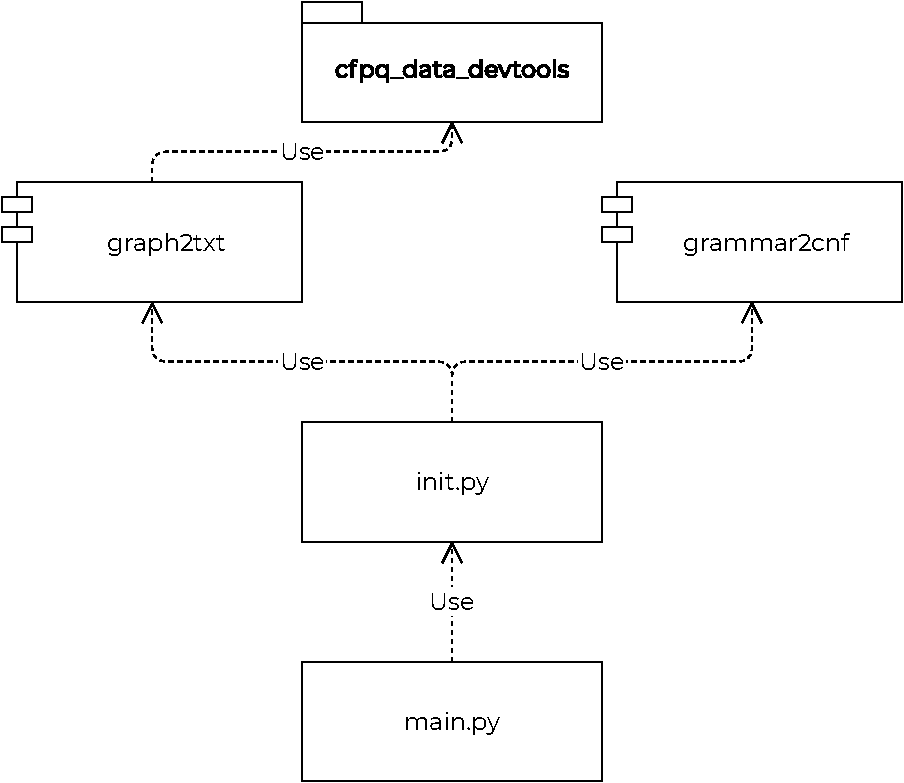
\includegraphics[width=0.9\textwidth]{img/architecture_old.pdf}
				\caption*{Рис. 3. Архитектура <<до>>} \label{fig:architecture_old}
			\end{figure}
        \end{column}

        \begin{column}{0.5\textwidth}
            \begin{figure}[hbt!]{\textwidth}
				\centering
				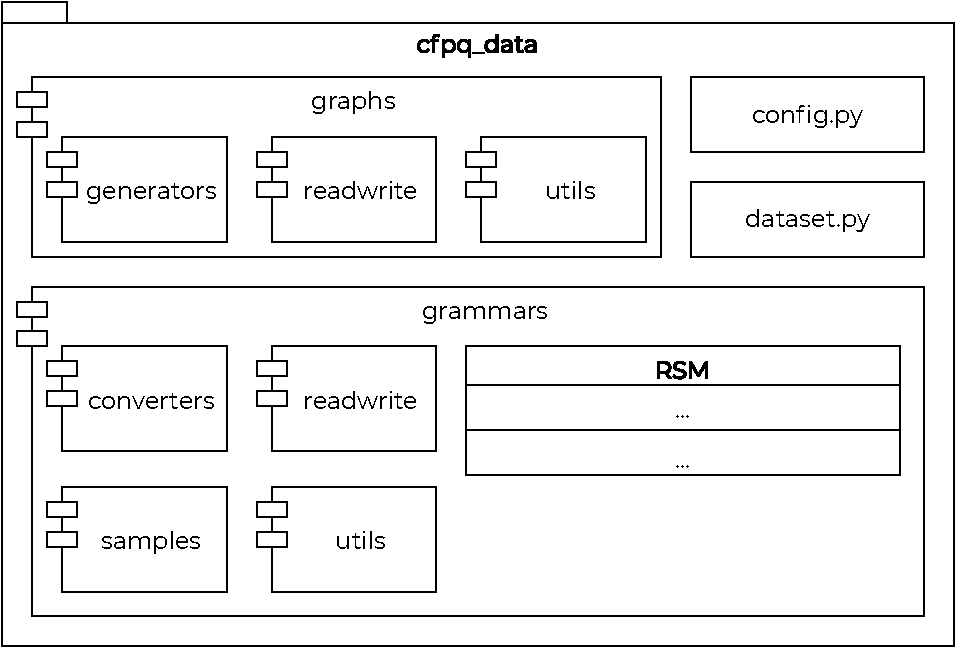
\includegraphics[width=0.9\textwidth]{img/architecture_new.pdf}
				\caption*{Рис. 4. Архитектура <<после>>} \label{fig:architecture_new}
			\end{figure}
        \end{column}
    \end{columns}
\end{frame}


\section{Эксперименты}
Для экспериментальных исследований были необходимы данные двух типов: последовательности РНК для подачи на вход синтаксическому анализатору и эталонные вторичные структуры для этих последовательностей --- и то, и другое было получено из популярной в исследовательских работах базы данных RNAstrand~\cite{andronescu2008rna}. Эта база представляет собой сборку тщательно отобранных и приведенных к единому формату данных сразу из нескольких надежных баз, содержащих цепочки РНК вместе с полученными методами лабораторного эксперимента или эволюционного анализа вторичными структурами. Из выгруженных данных были удалены дубликаты и образцы с неточностями в нуклеотидной цепи или же вторичной структуре --- таким образом была получена выборка из 800 последовательностей длин от 1 до 100, для которой были сгенерированы матрицы разбора и матрицы контактов, переведенные в черно-белые изображения.

Для оценки качества работы обученных на данных изображениях нейронных сетей были выбраны следующие метрики, посчитанные относительно попиксельной разницы между предсказанным и эталонным изображениями. Далее $TW$ (true white), $FW$ (false white) и $FB$ (false black) --- информация о том, сколько раз нейронная сеть приняла верное и сколько раз неверное решение по каждому пикселю (кроме диагональных) каждого изображения тестовой выборки.
\begin{itemize} 
    \item $Precision = \frac{TW}{TW + FW}$ (доля предсказанных контактов, которые действительно являются контактами в эталонном изображении).
    \item $Recall = \frac{TW}{TW + FB}$ (доля найденных нейронной сетью контактов среди всех искомых).
    \item $F1 = 2 * \frac{Precision * Recall}{Precision + Recall}$ (гармоническое среднее $Precision$ и $Recall$, используется как удобная объединяющая метрика).
\end{itemize}

При обучении нейросети была использована функция потерь, в основе построения которой лежит идея о максимизации метрики $F1$ с несколькими уточнениями. Во-первых, $F1$ дискретна, а функция ошибки должна быть дифференцируема вследствие вычисления на ней градиента. Во-вторых, передача среднего по выборке значения $1 - F1$ в качестве функции ошибки не гарантирует отсутствие большого разброса $Precision$ и $Recall$ как в пределах отдельно взятого изображения, так и в масштабах всей выборки, следствием чего будет нестабильность качества работы модели и высокая вероятность появления очень низкой точности результата для случайно взятого тестового образца. На основании данных соображений была реализована функция $F1\_loss$, представленная на рис.~\ref{loss}. Здесь дифференцируемость обеспечивается заменой сумм дискретных целочисленных значений на непрерывную сумму значений вероятности, а поддержка баланса между $Precision$ и $Recall$ для каждого изображения и для выборки в целом --- двумя пропорциональными величине разброса штрафными коэффициентами $k1$ и $k2$, накладываемыми на метрику $F1$.

\begin{figure}[h]
\begin{center}
\centering
\begin{python}
from keras import backend as K

def f1_loss(y_true, y_pred):
    #normalize pixels values to [0, 1]
    y_true, y_pred = K.minimum(y_true / 255, 1), K.minimum(y_pred / 255, 1)
    #calculate differentiable versions of TW, FW and FB
    tw = K.sum(K.cast(y_true * y_pred, 'float32'), axis=[1, 2, 3])
    fw = K.sum(K.cast((1 - y_true) * y_pred, 'float32'), axis=[1, 2, 3])
    fb = K.sum(K.cast(y_true * (1 - y_pred), 'float32'), axis=[1, 2, 3])
    #calculate precision and recall secure from zero division error
    precision = tw / (tw + fw + K.epsilon())
    recall = tw / (tw + fb + K.epsilon())
    #penalty coefficients for huge difference between precision and recall 
    #calculated for each image and whole dataset respectively
    k1 = 1 -  K.abs(precision - recall)
    k2 = 1 -  K.abs(K.mean(precision) - K.mean(recall))
    #calculate upgraded f1 score
    f1 = k1 * k2 * 2 * precision * recall / (precision + recall + K.epsilon()) 
    return 1 - K.mean(f1)
\end{python}
\caption{Функция потерь нейронной сети}
\label{loss}
\end{center}
\end{figure} 

Вследствие того, что количество обучаемых параметром используемой модели является достаточно большим относительно размера обучающей выборки, после каждого остаточного блока был добавлен слой Dropout, исключающий заданный процент случайных нейронов во время обучения. Кроме того, во всех сверточных слоях была применена регуляризация L2, которая, помимо уменьшения переобучения нейросети, оказывает положительное влияние на процесс поиска сложных закономерностей в данных. В качестве оптимизатора был использован адаптивный градиентный спуск (Adagrad), удобный для работы с разреженными данными, а также автоматически настраивающий скорость обучения.

Для сравнения результатов работы обученной модели с существующими в области аналогами был проведен анализ различных инструментов, предсказывающих вторичную структуру РНК, по следующим критериям: заявленная высокая точность результатов, возможность предсказания псевдоузлов, удобство использования и адекватное время работы. На основании данных соображений были отобраны шесть инструментов, основанных на различных подходах.
\begin{itemize}
    \item HotKnots --- минимизации свободной энергии через эвристический алгоритм~\cite{ren2005hotknots}.
    \item SPOT-RNA --- глубокое обучение, основанное на технике transfer learning~\cite{singh2019rna}.
    \item PknotsRG --- минимизация свободной энергии с использованием Turner energy rules~\cite{reeder2007pknotsrg}.
    \item RNAstructure --- минимизация свободной энергии с помощью динамического программирования~\cite{bellaousov2013rnastructure}.
    \item Ipknot --- поиск оптимальной вторичной структуры методом целочисленного программирования~\cite{sato2011ipknot}.
    \item Knotty --- алгоритм для минимизация свободной энергии, основанный на разреженном динамическом программировании~\cite{jabbari2018knotty}.
\end{itemize}

\subsection{Результаты}
Все тестовые запуски проводились на рабочей станции со следующими характеристиками.
\begin{itemize}
    \item Операционная система: Ubuntu 20.04.2 LTS.
    \item Центральный процессор: Intel Core i5-10210U CPU 1.60GHz.
    \item Графический процессор: NVIDIA GeForce MX250.
    \item Объем оперативной памяти: 7.5 GB.
\end{itemize}

На рис.~\ref{plot_f1} представлены значения метрики $F1$, показанные шестью вышеописанными инструментами на всей выборке из 800 образцов, а разработанной моделью (New-model) --- для различных разделений данных на обучающую и тестовую выборки (10\%:90\%, ..., 90\%:10\%). На графике видно, что при малых размерах обучающей выборки новая модель демонстрирует достаточно низкую точность, однако при увеличении выборки до 40\% результаты становятся сравнимыми с остальными подходами, а при максимальном объеме выборки (90\%) ---  лучшими в приведенном сравнении.

На рис.~\ref{plot_pr} показаны результаты аналогичного тестирования всех моделей по метрикам $Precision$ и $Recall$; здесь черная прямая $y=x$ символизирует оптимальное для рассматриваемой задачи положение этих метрик --- их равенство, --- а фиолетовая пунктирная линия указывает направление увеличения размера обучающей выборки для нашей модели от 10\% до 90\% с шагом в 10\%. Значения метрик для New-model расположены достаточно близко к желаемой прямой, что говорит о сбалансированности предсказаний разработанной нейросети. Кроме того, реализованный в данной работе алгоритм --- единственный на данном графике, имеющий $Recall$, больший, чем $Precision$: это произошло из-за того, что парсер находит значительную часть требуемых контактов, поэтому нейронная сеть, владея этой информацией еще до начала обучения, основной своей задачей имеет улучшение точности, а не полноты системы. Это делает наш подход несколько нетрадиционным относительно аналогов, которые, по всей видимости, сталкиваются с рядом проблем в процессе поиска контактов во вторичной структуре.

\begin{figure}[h]
\centering
\begin{subfigure}{.5\textwidth}
  \centering
  \fbox{\includegraphics[width=.95\linewidth]{pics/plot_f1.png}}
  \caption{Значения метрики $F1$}
  \label{plot_f1}
\end{subfigure}%
\begin{subfigure}{.5\textwidth}
  \centering
  \fbox{\includegraphics[width=.95\linewidth]{pics/plot_pr.png}}
  \caption{Значения метрик $Precision$ и $Recall$}
  \label{plot_pr}
\end{subfigure}
\caption{Сравнение разработанного подхода с аналогами}
\label{plot}
\end{figure}

Помимо точности, важной характеристикой алгоритма в области биоинформатики является время его работы, так как исследователям часто приходится работать с достаточно большими биологическими базами данных. В таблице~\ref{time} приведены замеры времени, потраченного всеми инструментами на обработку 100 цепочек РНК различных длин из промежутка от 1 до 100. Несмотря на то, что разные подходы могут предполагать разные сценарии использования (обработка одной или нескольких последовательностей, вывод ответа через интерфейс командной строки или в специальный файл, а также сохранение результатов в различных форматах), одним из традиционных вариантов является обработка файла в формате fasta, содержащего набор последовательностей с метаданными, и последующее сохранение результата в одном из общепринятых форматов (например, dot-bracket или bpseq). Для данного сценария и был произведен сравнительный анализ производительности подходов: файл с последовательности был преобразован в необходимые для всех инструментов входные форматы, выходные же форматы были оставлены без изменений. В таблице~\ref{time} представлены средние значения для десяти прогонов в секундах, упорядоченные по возрастанию времени. Интсрументы Ipknot, Hotknots, PknotsRG, RNAstructure и Knotty работают только на CPU, SPOT-RNA имеет и CPU, и GPU-реализации, а для нашего подхода как алгоритм синтаксического анализа (PA), так и нейронная сеть (NN) используют GPU. Можно увидеть, что New-model значительно проигрывает по времени большинству аналогов и наиболее времязатратной операцией здесь является синтаксический анализ, занимающий почти 80\% от общего времени работы.

\begin{table}[h]
\centering
\begin{tabular}{|p{5.5cm}||p{4.5cm}|}
\hline
\textbf{Tool} & \textbf{Time, s} \\ \hline\hline
Ipknot & 0.8 \\ \hline
RNAstructure & 10.3 \\ \hline
PknotsRG & 14.9 \\ \hline
Hotknots & 37.0 \\ \hline
SPOT-RNA (GPU) & 67.8 \\ \hline
New-model (PA + NN) & 103.1 (80.7 + 22.4) \\ \hline
SPOT-RNA (CPU) & 109.7 \\ \hline
Knotty & 282.8 \\ \hline
\end{tabular}
\end{table}

Подводя итоги, экспериментальные исследования показали работоспособность разработанного подхода применительно к задаче предсказания вторичной структуры РНК даже в сравнении с лучшими инструментами в области. Высокая точность уже полученных результатов вместе с общей гибкостью подхода и обширными возможностями для дальнейших экспериментов позволяют полагать, что предложенные в данной работе идеи имеют значительный потенциал. Однако на данный момент наш проект по большей части исследовательский --- для создания полноценного инструмента требуется тщательный анализ качества всех обученных на различного размера выборках моделей с целью выбора оптимальной, а также, несомненно, повышение производительности подхода, в частности, ускорение синтаксического анализатора.

\section{Заключение}
\section{Conclusion}

Conclusion, current state, results.

Future work. Library extension up to full GraphBLAS API implementation.

LaGraph on F\# .NET.

Evaluation. Comparison with other implementations on different devices.
Manual implementation versus translation.  

Another direction of future work is Brahma.FSharp improvements. 
First of all, it is necessary to support discriminated unions to make it possible to express custom semirings such as \texttt{Min-Plus}, as presented in listing~\ref{lst_example}. 

Also, it is necessary to add high-level abstractions for asynchronous programming, and for multi-GPU programming.
Such mechanisms can be naturally expressed in F\# with native primitives for asynchronous programming.

fusion and other optimizations.

% \nocite{*}
\setmonofont[Mapping=tex-text]{CMU Typewriter Text}
\bibliographystyle{ugost2008ls}
\bibliography{vkr}
\end{document}
